\problemname{Brevoptimering}
The Programming Olympiad committee, consisting of $N$ people, is sending out envelopes with posters for the qualification round to all schools.
To speed up the process, they have divided up the tasks that need to be done.
The tasks include writing addresses, putting on stamps, inserting the posters, and sealing the envelopes.
When a person is done with an envelope, it is passed on to some other person.
It is not going as fast as they had hoped, and therefore they wonder who could work faster.

Each person $p$ has their own maximum production rate $M_p$ envelopes per second.
If we let $I_p$ be the number of envelopes sent to person $p$ per second and let $U_p$ be the number of envelopes they finish per second, then $U_p = \min(I_p, M_p)$.
A person thus does not finish more than $M_p$ envelopes per second, even if they receive more to work on.
Each person also has a number of people to whom they send the envelopes they finish.
They do not have to send the same number of envelopes to each person; each recipient gets a certain percentage of the envelopes $p$ sends.
The people to whom nobody sends envelopes, and who are thus at the beginning of the production line, have $I_p = \infty$, and therefore $U_p = M_p$ (they have an infinite pile of envelopes to draw from).
Some people do not pass on any envelopes at all; they just put them in a pile next to themselves when they are done.

For which people does $U_p = M_p$ hold, i.e.\ who works at their maximum production rate?

\section*{Input}
The first line contains an integer $N$ ($1 \le N \le 10^5$), the number of people.
The next $N$ lines describe the people. Line $i$ first contains the integer $M_i$, the maximum production rate for person $i$ ($1 \le M_i \le 10^5$).
Then follows an integer $k$, and then $k$ pairs of integers $j$ $w$, meaning that person $i$ sends $w$ percent of their envelopes to person $j$ ($1 \le w \le 100$, $1 \le j \le N, i \neq j$).
No $j$ can appear more than once on a given line, and the sum of the $w$ values on the line will be $100$, unless $k = 0$.

Let $S$ denote the sum of all $k$ values. Then $0 \le S \le 10^5$.

The production chain is designed in such a way that no person can receive back an envelope they have already worked on.

\section*{Output}
Print a line with all $i$ satisfying $U_p = M_p$, in increasing order.

It is guaranteed that if $U_p = M_p$ then this will hold with margin; more specifically $I_p - M_p > 10^{-4}$.
Conversely, if $U_p \neq M_p$ then there will be margin the other way: $M_p - I_p > 10^{-4}$.

\section*{Scoring}
Your solution will be tested on a set of test groups.
To earn points for a group, you must pass all test cases in that group.

\noindent
\begin{tabular}{| l | l | l |}
\hline
Group & Points & Constraints \\ \hline
$1$    & $12$       &  Each person sends envelopes to at most one person (i.e.\ $k \leq 1$) and receives envelopes from at most one person \\ \hline
$2$    & $17$       &  Each person receives envelopes from exactly one other person, except person $1$ who receives from nobody \\ \hline
$3$    & $21$       &  If person $i$ sends to person $j$ then $i < j$ \\ \hline
$4$    & $25$       &  $N, S \le 10$ \\ \hline
$5$    & $25$       &  No additional constraints. \\ \hline
\end{tabular}

\section*{Explanation of Samples}
Below are three graphs representing the three samples. Each person is represented by a node. On each edge, the number of envelopes sent is written in the unit eps (envelopes per second).

Note that in test group $1$, only sample $1$ could occur; in test group $2$, only sample $2$; and in test group $3$, only sample $3$.
In test groups $4$ and $5$, all three samples could occur.
\begin{figure}
	\centering
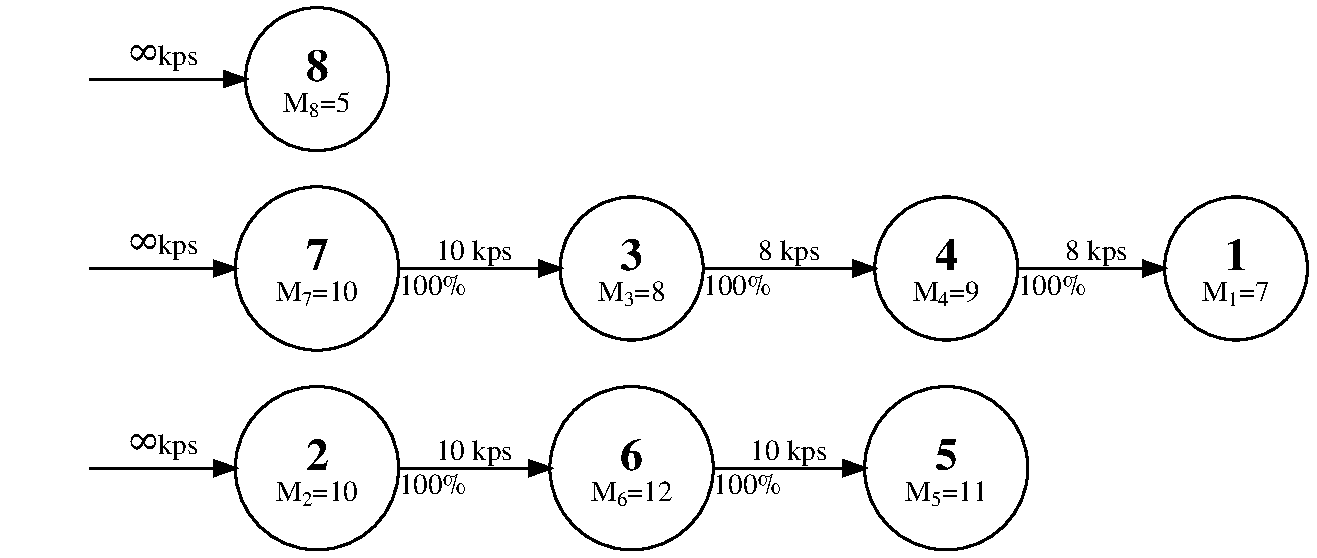
\includegraphics[width=0.8\textwidth]{sample1}
\caption{Sample $1$}
\end{figure}
\begin{figure}
	\centering
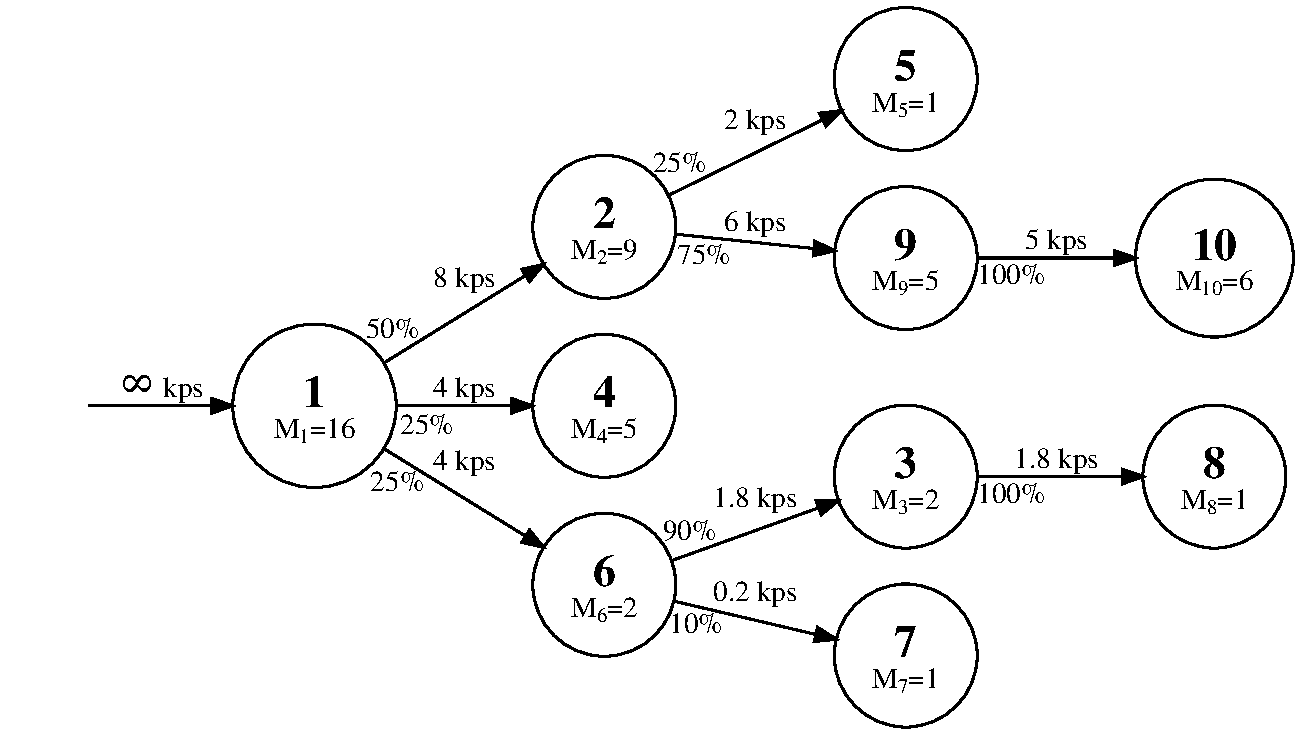
\includegraphics[width=0.8\textwidth]{sample2}
\caption{Sample $2$}
\end{figure}
\begin{figure}
	\centering
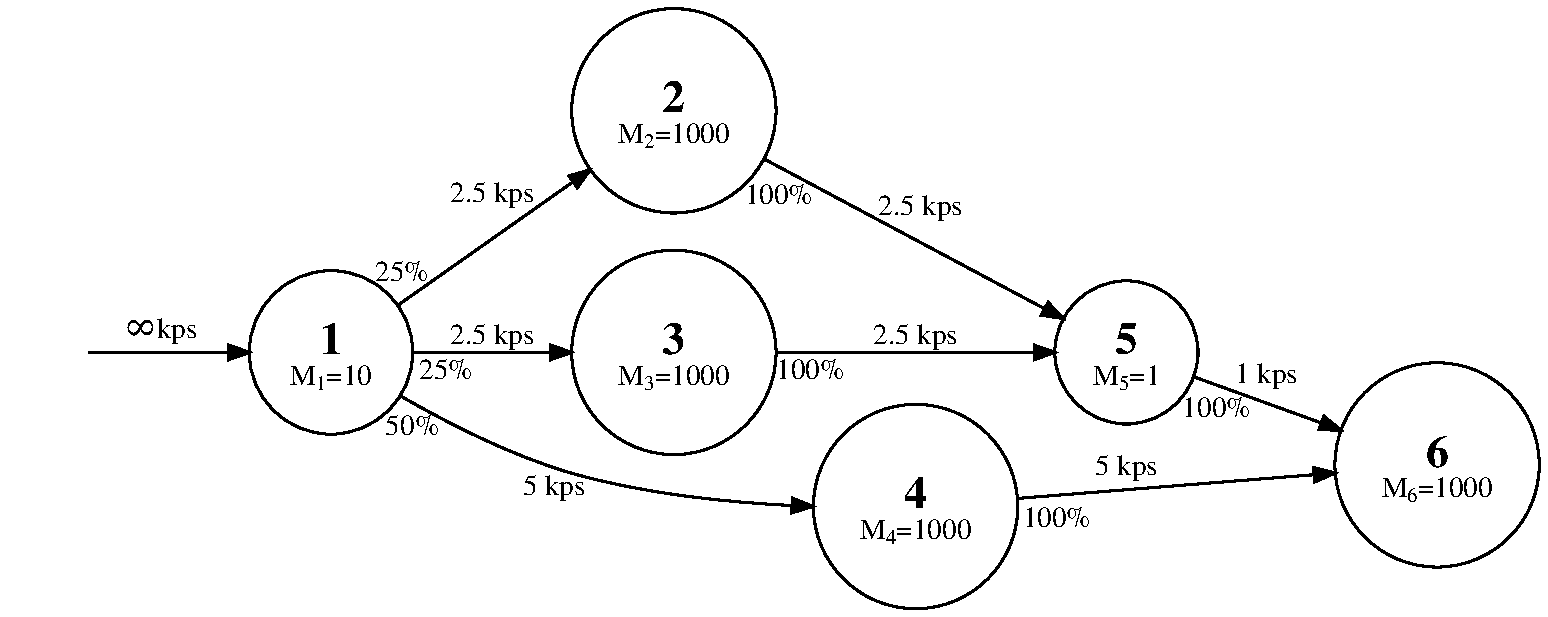
\includegraphics[width=0.8\textwidth]{sample3}
\caption{Sample $3$}
\end{figure}
